\pgfplotsset{width=7cm,compat=1.3}
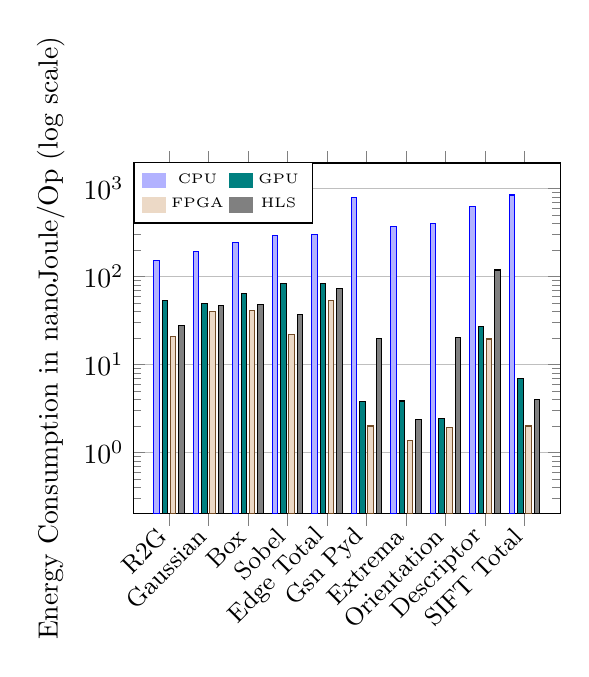
\begin{tikzpicture}
\begin{axis}[
    legend style={font=\tiny},
    ybar=1pt,
    bar width =2pt,
    ymin=0.2,ymax=850,
    enlarge y limits={upper=0.15},
     ymode=log,
    legend image code/.code={\draw[#1, draw=none] (0cm,-0.1cm) rectangle (0.3cm,0.1cm);
                },
    ymajorgrids = true,
    legend style={at={(-0.00000009,0.915)},
                   anchor=west,legend columns=2},
    ylabel={Energy Consumption in nanoJoule/Op (log scale) },
    symbolic x coords={R2G,Gaussian,Box,Sobel,Edge Total,Gsn Pyd,Extrema,Orientation,Descriptor,SIFT Total},
    xtick=data,
    %nodes near coords,
    nodes near coords style={font=\tiny, anchor=west,rotate=90,inner
    xsep=0.5pt},
    x tick label style = {font=\small, rotate=45, anchor=east},
    ]

\addplot coordinates {(R2G,151) (Gaussian,193)  (Box,246) (Sobel,290) (Edge Total,304) (Gsn Pyd,801) (Extrema,369) (Orientation,401) (Descriptor,620) (SIFT Total, 848)};%CPU

\addplot [fill=teal!]  coordinates {(R2G,54) (Gaussian,50)  (Box,64) (Sobel,83) (Edge Total, 83) (Gsn Pyd,3.76)(Extrema,3.85) (Orientation,2.41) (Descriptor,27.3)  (SIFT Total, 6.92)  };%GPU

\addplot coordinates {(R2G,21) (Gaussian,40)  (Box,41) (Sobel,22) (Edge Total, 53) (Gsn Pyd,2.00)(Extrema,1.38) (Orientation,1.90) (Descriptor,19.5)  (SIFT Total, 2) };%FPGA

\addplot coordinates {(R2G,28) (Gaussian,47)  (Box,48) (Sobel,37) (Edge Total, 73) (Gsn Pyd,19.8) (Extrema,2.36) (Orientation,20.2) (Descriptor,119)  (SIFT Total, 4) };%HLS

\legend{CPU,GPU,FPGA,HLS}
\end{axis}
\end{tikzpicture}